\section{\textbf{\textsc{RemapRoute}}}
\label{sec:remap}

Agora apresentamos nosso algoritmo para remapeamento local de mudanças
de caminho implementado no \rmprt{}.  O algoritmo recebe como entrada a
rota antiga observada antes da mudança de roteamento $C(t_{i-1})$ e o
salto $s^\prime$ do roteador onde a mudança foi detectada,
$C(t_i)[s^\prime] \ne C(t_{i-1})[s^\prime]$.  Para remapear a mudança de
rota, \rmprt{} opera em duas etapas: primeiro ele localiza onde a
mudança aconteceu (\secstr~\ref{sec:remap.locate}) e depois faz o
remapeamento local da mudança (\secstr~\ref{sec:remap.local}).

O processo de localização e remapeamento da mudança de rota envolve
remapear saltos da rota atual e compará-los com saltos na rota antiga.
Para remapear cada salto, o \rmprt{} envia múltiplas sondas, modificando
sistematicamente os campos do cabeçalho IP como o Paris
traceroute~\cite{augustin07, veitch09balancer}, para identificar
roteadores que fazem balanceamento de carga.

\subsection{Localização da mudança de roteamento}
\label{sec:remap.locate}

O \rmprt{} parte de um salto $s^\prime$ onde o roteador na rota atual é
diferente do roteador na rota antiga, $C(t_i)[s^\prime] \ne
C(t_{i-1})[s^\prime]$.  Se o roteador da rota atual no salto $s^\prime$
não pertencer à rota antiga, $C(t_i)[s^\prime] \notin C(t_{i-1})$, então
$s^\prime$ é um dos saltos envolvidos na mudança de caminho e podemos
passar para a próxima etapa para remapear a mudança
(\secstr~\ref{sec:remap.local}).

Se o roteador da rota atual no salto $s^\prime$ pertencer à rota antiga
em outro salto $s^{\prime\prime}$, $C(t_i)[s^\prime] =
C(t_{i-1})[s^{\prime\prime}]$, então temos uma mudança de roteamento em
saltos anteriores a $s^\prime$ que adicionou ou removeu roteadores na
rota.  A \figstr~\ref{fig:remap.example} mostra um exemplo de uma
mudança de roteamento onde o roteador $d$ foi substituído por dois
roteadores $x$ e $y$.  Uma sonda para o sétimo salto detecta uma mudança
de roteamento pois a resposta da sonda vem do roteador $g = C(t_i)[7]$,
que não é a resposta esperada na rota antiga, $h = C(t_{i-1})[7]$.

\begin{figure}[h] % {{{
\begin{center}
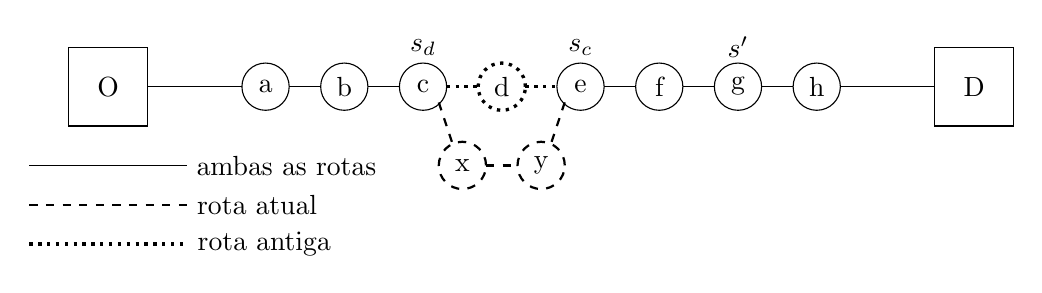
\begin{tikzpicture}
\draw (-1-0.5,-0.5) -- (-1-0.5,0.5) -- (-1+0.5,0.5) -- (-1+0.5,-0.5) --
cycle;
\node at (-1,0) {O};
%
\draw (10-0.5,-0.5) -- (10-0.5,0.5) -- (10+0.5,0.5) -- (10+0.5,-0.5) --
cycle;
\node at (10,0) {D};
%
\draw (1,0) circle (3mm);
\draw (2,0) circle (3mm);
\draw (3,0) circle (3mm);
\draw[dotted, very thick] (4,0) circle (3mm);
\draw (5,0) circle (3mm);
\draw (6,0) circle (3mm);
\draw (7,0) circle (3mm);
\draw (8,0) circle (3mm);
\node at (1,0) {a};
\node at (2,0) {b};
\node at (3,0) {c};
\node at (4,0) {d};
\node at (5,0) {e};
\node at (6,0) {f};
\node at (7,0) {g};
\node at (8,0) {h};
%
\foreach \i in {1,...,2}
{ \draw (\i+0.3,0) -- (\i+1-0.3,0); }
\foreach \i in {5,...,7}
{ \draw (\i+0.3,0) -- (\i+1-0.3,0); }
\draw[dotted, very thick] (3+0.3,0) -- (4-0.3,0);
\draw[dotted, very thick] (4+0.3,0) -- (5-0.3,0);
\draw (-1+0.5,0) -- (1-0.3,0);
\draw (8+0.3,0) -- (10-0.5,0);
%
\draw[dashed, thick] (3.5,-1) circle (3mm);
\draw[dashed, thick] (4.5,-1) circle (3mm);
\node at (3.5,-1) {x};
\node at (4.5,-1) {y};
\draw[dashed, thick] (3.2,-0.2) -- (3.4,-0.8);
\draw[dashed, thick] (4.8,-0.2) -- (4.6,-0.8);
\draw[dashed, thick] (3.5+0.3,-1) -- (4.5-0.3,-1);
%
\node at (3, 0.5) {$s_d$};
\node at (5, 0.5) {$s_c$};
\node at (7, 0.5) {$s^\prime$};
%
\draw (-2,-1) -- (0,-1) node[right] {ambas as rotas};
\draw[dashed, thick] (-2,-1.5) -- (0,-1.5) node[right] {rota atual};
\draw[dotted, very thick] (-2,-2) -- (0,-2) node[right] {rota antiga};
%
\end{tikzpicture}
\end{center}
\caption{Exemplo de mudança de roteamento com adição de roteadores à
rota.}
\label{fig:remap.example}
\end{figure} % }}}

Para encontrar um roteador envolvido na mudança de caminho, i.e., um
roteador na rota atual que não está presente na rota antiga, o \rmprt{}
faz uma busca binária no caminho.  O \rmprt{} inicializa $s_\mathrm{esq}
= 0$ e $s_\mathrm{dir} = s^\prime$.  A cada iteração da busca, o
\rmprt{} remapeia o salto $s = (s_\mathrm{esq} + s_\mathrm{dir})/2$ e
procura o roteador no salto $s$ da rota atual na rota antiga.  Se o
roteador no salto $s$ da rota atual não pertencer à rota antiga,
$C(t_i)[s] \notin C(t_{i-1})$, a busca termina e passamos para a etapa
de remapeamento.  Se o roteador no salto $s$ da rota atual estiver no
salto $s$ da rota antiga, $C(t_i)[s] = C(t_{i-1})[s]$, então a mudança
está à direita de $s$ e fazemos $s_\mathrm{esq} = s$.  Se o roteador no
salto $s$ da rota atual estiver em outro salto $s^{\prime\prime}$ na
rota antiga, $C(t_i)[s] = C(t_{i-1})[s^{\prime\prime}]$, a mudança está
à esquerda de $s$ e fazemos $s_\mathrm{dir} = s$.

Não temos como comparar a rota atual com a rota antiga se o roteador no
salto $s$ não responde a sondas.  Neste caso tomamos a decisão
conservadora de decrementar $s$ e continuar a busca no salto anterior,
sem alterar $s_\mathrm{esq}$ e $s_\mathrm{dir}$.  

Se uma mudança de caminho apenas remove saltos da rota antiga, então não
existe salto na rota atual que não pertença à rota antiga.  Neste caso,
o processo de busca termina com $s_\mathrm{esq} = s_\mathrm{dir} + 1$ e
nenhum remapeamento é necessário (\secstr~\ref{sec:remap.local}).

\subsection{Remapeamento local}
\label{sec:remap.local}

O remapeamento local parte de um salto $s$ onde o roteador na rota atual
não pertence à rota antiga, $C(t_i)[s] \notin C(t_{i-1})$.  O \rmprt{}
remapeia sequencialmente os saltos da rota atual posteriores a $s$ até
encontrar o salto de convergência $s_c > s$ com um roteador que pertence
à rota antiga, $C(t_i)[s_c] \in C(t_{i-1})$.  Se uma das rotas não chega
até o destino, o salto de convergência pode não existir.  Neste caso, o
\rmprt{} remapeia a rota atual até o destino ou até o último salto
alcançável.  Se o caminho não chega até o destino, o \rmprt{} identifica
o último salto alcançável após encontrar três saltos consecutivos que
não respondem a sondas (igual o traceroute).

De forma similar, o \rmprt{} remapeia sequencialmente os saltos da rota
atual anteriores a $s$ até encontrar o salto de divergência $s_d < s$
com um roteador que pertence à rota antiga, $C(t_i)[s_d] \in
C(t_{i-1})$.  No pior caso, a busca pelo salto de divergência termina na
origem, que pertence a qualquer rota no caminho.  Se o salto $s_d$ não
for idêntico nas duas rotas, $C(t_i)[s_d] \ne C(t_{i-1})[s_d]$, então
existe outra mudança de roteamento anterior a $s_d$ e voltamos à
primeira etapa (\secstr~\ref{sec:remap.locate}), fazendo $s^\prime =
s_d$, para localizá-la e depois remapeá-la.  Esse processo é realizado
recursivamente até que não reste nenhuma mudança para remapear.
%
O remapeamento dos roteadores nos saltos entre $s_d$ e $s_c$ precisa ser
sequencial pois todos estão envolvidos na mudança de roteamento.  Para
mudanças de roteamento que apenas removem saltos, temos $s_d =
s_\mathrm{esq}$ e $s_c = s_\mathrm{dir}$ e nenhum remapeamento é
necessário.

\subsection{Exemplo}

Considere que a mudança de roteamento mostrada na
\figstr~\ref{fig:remap.example} tenha sido detectada com uma sonda para
o quinto salto no caminho.  Temos $C(t_{i-1})[5] = f$ e $C(t_i)[5] = e$.
Como $e \in C(t_{i-1})$, um nó foi inserido antes do quinto salto e o
\rmprt{} inicia uma busca binária para identificar o local da mudança.
O \rmprt{} começa remapeando o segundo salto, onde $C(t_{i-1})[2] =
C(t_i)[2] = c$, indicando que a inserção foi realizada entre o segundo e
o quinto salto.  O \rmprt{} remapeia então o terceiro salto, onde
$C(t_{i-1})[3] = d$ e $C(t_i)[3] = x$.  Como $x \notin C(t_{i-1})$ o
\rmprt{} passa para a fase de remapeamento local da mudança, onde
remapeia o quarto salto e termina.
